\par O primeiro modelo com dependência que vamos discutir é chamado de ``Percolação $2k$ Dependente''. Este é um modelo de percolação (dependente) de elos induzido por um modelo de percolação (independente) de vértices. Para defini-lo, comece, como feito na Seção \ref{Bernoulli-percolation}, com um grafo $d$ dimensional $\LX^d = (\ZX^d, \text{E}^d)$, com $\ZX^d$ conjunto de vértices e $\text{E}^d$ conjunto de elos tal que $\text{E}^d = \left\{(x, y) \in \ZX^d \times \ZX^d : \sum_{i = 1}^{d} |x_i - y_i| = 1\right\}$.

\par Para o modelo de elos, defina um primeiro espaço de probabilidade $(\Omega, \FX, \mu_p)$ onde $\Omega = \prod_{e \in \text{E}^d} \{0, 1\}$, com $w = (\omega_e : e \in \text{E}^d) \in \Omega$, tal que $\omega_e = 0$ para $e$ ``fechado'' e $\omega_e = 1$ para $e$ ``aberto'', $\FX = \sigma($cilindros finito-dimensionais$)$ e $\mu_p: \FX \longrightarrow [0, 1]$ medida de probabilidade. De maneira similar, para o modelo de vértices, defina um segundo espaço de probabilidade $(\Xi, \GX, \PX_p)$ onde $\Xi = \prod_{x \in \ZX^d}\{0, 1\}$, com $\xi = (\xi_x : x \in \ZX^d)$, $\GX = \sigma($cilindros finito-dimensionais$)$ e $\PX_p(\xi) = \prod_{x:\xi_x = 1}p\prod_{x:\xi_x = 0}(1-p)$. Finalmente, como forma de, indiretamente, determinar a medida $\mu_p$, diga que, para $k \in \NX$ fixo, $\omega_e = 1$ se existe $x \in \ZX^d$ tal que $\xi_x = 1$ e $e \in \Lambda_k(x)$; ou seja, um elo $e$ está aberto se pertence a alguma caixa $\Lambda_k$ centrada em $x$ tal que $\xi_x = 1$. Formalmente, se $f: \Xi \longrightarrow \Omega$ é tal que $f^{-1}(A) = \{\xi \in \Xi : f(\xi) \in A\}$, $\forall A \in \FX$, então $\mu_p(A) = (f_{*}(\PX_p))(A) = \PX_p(f^{-1}(A))$, $\forall A \in \FX$. A Figura \ref{configuracao-2k} mostra o recorte de uma possível configuração desse modelo em $\LX^2$.

\par Para ``Percolação $2k$'' como acabamos de definir, note que existe dependência para os estados dos elos; já que o conhecimento sobre o estado de um elo arbitrário $e$ nos dá alguma informação sobre os estados de seus vizinhos. Porém, veja que, para dois elos $e = (x, y), ~f = (w, z) \in \text{E}^d$, se $w, z \not\in \Lambda_k(x) \cup \Lambda_k(y)$, então $\text{COV}_p(\omega_e, \omega_f) = 0$, onde $\text{COV}_p(\cdot, \cdot)$ é \textit{covariância} com respeito à medida $\mu_p$. Por causa dessa característica, esse modelo é conhecido como ``modelo dependente de curto alcance''.\vspace{9pt}

\begin{figure*}[!htbp]
	\centering
	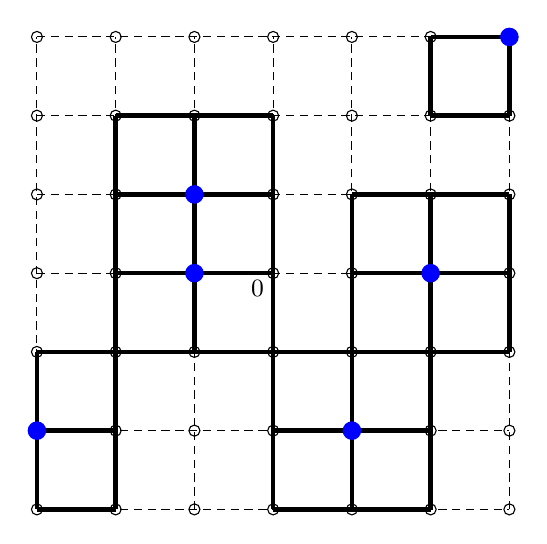
\begin{tikzpicture}[scale = 1]

\node[black] at (-0.20, -0.20) {{\small $0$}};

\draw[densely dashed, black] (-3, -2) -- (3, -2);
\draw[densely dashed, black] (-3, -1) -- (3, -1);
\draw[densely dashed, black] (-3,  0) -- (3,  0);
\draw[densely dashed, black] (-3,  1) -- (3,  1);
\draw[densely dashed, black] (-3,  2) -- (3,  2);
\draw[densely dashed, black] (-2, -3) -- (-2, 3);
\draw[densely dashed, black] (-1, -3) -- (-1, 3);
\draw[densely dashed, black] (0,  -3) -- (0,  3);
\draw[densely dashed, black] (1,  -3) -- (1,  3);
\draw[densely dashed, black] (2,  -3) -- (2,  3);
\draw[densely dashed, black] (-3, -3) -- (3, -3);
\draw[densely dashed, black] (-3,  3) -- (3,  3);
\draw[densely dashed, black] (-3, -3) -- (-3, 3);
\draw[densely dashed, black] ( 3, -3) -- (3,  3);


\draw[solid, black, ultra thick] (-1,-1) -- (-1,2);
\draw[solid, black, ultra thick] (-2,-1) -- (-2,2);
\draw[solid, black, ultra thick] ( 0,-1) -- ( 0,2);

\draw[solid, black, ultra thick] (-2, 2) -- ( 0,2);
\draw[solid, black, ultra thick] (-2, 1) -- ( 0,1);
\draw[solid, black, ultra thick] (-2, 0) -- ( 0,0);
\draw[solid, black, ultra thick] (-2,-1) -- (0,-1);

\draw[solid, black, ultra thick] (3, 1) -- (3,-1);

\draw[solid, black, ultra thick] (2, 1) -- (2,-3);
\draw[solid, black, ultra thick] (1, 1) -- (1,-3);

\draw[solid, black, ultra thick] (1, 1) -- (3, 1);
\draw[solid, black, ultra thick] (1, 0) -- (3, 0);
\draw[solid, black, ultra thick] (1,-1) -- (3,-1);

\draw[solid, black, ultra thick] (0,-1) -- (2,-1);
\draw[solid, black, ultra thick] (0,-2) -- (2,-2);
\draw[solid, black, ultra thick] (0,-3) -- (2,-3);

\draw[solid, black, ultra thick] (0,-1) -- (0,-3);

\draw[solid, black, ultra thick] (3, 3) -- (3, 2);
\draw[solid, black, ultra thick] (3, 2) -- (2, 2);
\draw[solid, black, ultra thick] (2, 2) -- (2, 3);
\draw[solid, black, ultra thick] (2, 3) -- (3, 3);

\draw[solid, black, ultra thick] (-3, -1) -- (-3, -3);
\draw[solid, black, ultra thick] (-2, -1) -- (-2, -3);

\draw[solid, black, ultra thick] (-3, -1) -- (-2, -1);
\draw[solid, black, ultra thick] (-3, -2) -- (-2, -2);
\draw[solid, black, ultra thick] (-3, -3) -- (-2, -3);


\draw[black] (-2, -2) circle (2pt);
\draw[black] (-2, -1) circle (2pt);
\draw[black] (-2,  0) circle (2pt);
\draw[black] (-2,  1) circle (2pt);
\draw[black] (-2,  2) circle (2pt);
\draw[black] (-1, -2) circle (2pt);
\draw[black] (-1, -1) circle (2pt);
\draw[fill, blue] (-1,  0) circle (3.15pt);
\draw[fill, blue] (-1,  1) circle (3.15pt);
\draw[black] (-1,  2) circle (2pt);
\draw[black] (0,  -2) circle (2pt);
\draw[black] (0,  -1) circle (2pt);
\draw[black] (0,   0) circle (2pt);
\draw[black] (0,   1) circle (2pt);
\draw[black] (0,   2) circle (2pt);
\draw[fill, blue] (1,  -2) circle (3.15pt);
\draw[black] (1,  -1) circle (2pt);
\draw[black] (1,   0) circle (2pt);
\draw[black] (1,   1) circle (2pt);
\draw[black] (1,   2) circle (2pt);
\draw[black] (2,  -2) circle (2pt);
\draw[black] (2,  -1) circle (2pt);
\draw[fill, blue] (2,   0) circle (3.15pt);
\draw[black] (2,   1) circle (2pt);
\draw[black] (2,   2) circle (2pt);

\draw[black] (3, -3) circle (2pt);
\draw[black] (3, -2) circle (2pt);
\draw[black] (3, -1) circle (2pt);
\draw[black] (3,  0) circle (2pt);
\draw[black] (3,  1) circle (2pt);
\draw[black] (3,  2) circle (2pt);
\draw[fill, blue] (3,  3) circle (3.15pt);

\draw[black] (-3, -3) circle (2pt);
\draw[fill, blue] (-3, -2) circle (3.15pt);
\draw[black] (-3, -1) circle (2pt);
\draw[black] (-3,  0) circle (2pt);
\draw[black] (-3,  1) circle (2pt);
\draw[black] (-3,  2) circle (2pt);
\draw[black] (-3,  3) circle (2pt);

\draw[black] (-2 ,3) circle (2pt);
\draw[black] (-1 ,3) circle (2pt);
\draw[black] ( 0 ,3) circle (2pt);
\draw[black] ( 1 ,3) circle (2pt);
\draw[black] ( 2 ,3) circle (2pt);

\draw[black] (-2 ,-3) circle (2pt);
\draw[black] (-1 ,-3) circle (2pt);
\draw[black] ( 0 ,-3) circle (2pt);
\draw[black] ( 1 ,-3) circle (2pt);
\draw[black] ( 2 ,-3) circle (2pt);


\end{tikzpicture}
	\caption{Configuração possível para o modelo de Percolação $2k$ Dependente com $k = 1$ em recorte de $\LX^2$.}
	\label{configuracao-2k}
\end{figure*}

Utilizando o resultado de Liggett, Schonmann e Stacey em \cite{liggett1997domination}, temos que, para um modelo de percolação com dependência finita em $\LX^d$ com $d \geq 2$, existe $p_c = p_c(d) \colonequals \sup \{p: \theta(p) = 0\} < 1$ (isto é, existe transição de fase para o modelo de Percolação $2k$ Dependente), onde, de novo, $\theta: [0, 1] \longrightarrow [0, 1]$ é função que mapeia $p \mapsto \mu_p(\{\omega \in \Omega : |C_0(\omega)| = +\infty\})$. Nesse sentido, como fizemos na Subseção \ref{subsection-exp-decay}, nos interessa estudar o comportamento da função $\theta(p)$ para $p < p_c$ e $p > p_c$. O teorema abaixo, similar ao Teorema \ref{exp-decay}, nos dá um resultado desse tipo.

\begin{mythm} \label{exp-decay-2k}
	No modelo de Percolação $2k$ Dependente em $\LX^d$, existe $p_c = p_c(d, k)$ tal que vale
	\begin{enumerate}[1.]
		\item Para $p < p_c$, existe um $c_p > 0$ tal que para todo $n \geq 1$, $\mu_p(0 \leftrightarrow \partial\Lambda_n) \leq e^{-c_p \, n}$.
		\item Para $p > p_c$, existe um $c > 0$ tal que $\mu_p(|C_0(\omega)| = +\infty) \geq c \, (p - p_c)$.
	\end{enumerate}
\end{mythm}

\texttt{Demonstração:}

A estratégia adotada será muito parecida com a demonstração feita para o Teorema \ref{exp-decay}; de fato, considere uma família de algoritmos $\text{\textbf{T}}$ similar àquela definida para o Lema \ref{lem-infl}. O algoritmo $\text{\textbf{T}}$ para $f_n(\xi) \colonequals \IX_{0 \overset{\omega}{\leftrightarrow}\partial\Lambda_n}(\xi)$ irá revelar, através de um processo de exploração de vértices, o aglomerado de $\partial\Lambda_{s}$, com $1 \leq s \leq n$. Nesse caso, perceba que $\text{\textbf{T}}$ deve explorar, primeiro, todos os vértices $x \in \Lambda_n$ tal que $\partial\Lambda_k(x)$ está conectada, através de um caminho aberto no processo de percolação de elos, a $\partial\Lambda_s$ (notação: $\partial\Lambda_k(x) \overset{\omega}{\leftrightarrow} \partial\Lambda_s$). A Figura \ref{exploracao-2k} apresenta um esboço do algoritmo de exploração $\text{\textbf{T}}$ que acabamos de descrever.

\begin{figure*}[!htbp]
	\centering
	\begin{tikzpicture}[scale = 1.50]

	\begin{scope}	
		\clip (0.60, 0) to[out = 86, in = 135] (1.25, 0.75) to[out = -45, in = 135] (1.75, -0.5) to[out = -45, in = -95] (0.60, 0); % Área limitada
		\draw[pattern = north east lines, pattern color = black!30] (-2 , -2) rectangle (2, 2); % Área total
	\end{scope}
	
	\begin{scope}	
		\draw[pattern = north west lines, pattern color = black!30] (1.10, -1.20) rectangle (1.90, -0.40); % Área total
	\end{scope}

	\draw[solid, black] (-2,  2) -- ( 2,  2);
	\draw[solid, black] ( 2,  2) -- ( 2, -2);
	\draw[solid, black] ( 2, -2) -- (-2, -2);
	\draw[solid, black] (-2, -2) -- (-2,  2);
	
	\draw[dashed, black] (-0.75,  0.75) -- ( 0.75,  0.75);
	\draw[dashed, black] ( 0.75,  0.75) -- ( 0.75, -0.75);
	\draw[dashed, black] ( 0.75, -0.75) -- (-0.75, -0.75);
	\draw[dashed, black] (-0.75, -0.75) -- (-0.75,  0.75);
	
	\draw[solid, black] ( 1.10, -0.40) -- ( 1.90, -0.40);
	\draw[solid, black] ( 1.90, -0.40) -- ( 1.90, -1.20);
	\draw[solid, black] ( 1.90, -1.20) -- ( 1.10, -1.20);
	\draw[solid, black] ( 1.10, -1.20) -- ( 1.10, -0.40);
	
	\draw[fill, black] (1.50, -0.80) circle (1.25pt);
	\draw[black] ( 0,  0) circle (1.75pt);
	\node[black] at (0, -.30) {{\small $0$}};
	\node[black] at (1.88, -2.20) {{\small $\Lambda_n$}};
	\node[black] at (0.63, -0.95) {{\small $\Lambda_s$}};
%	\node[red] at (1.25,  1.10) {{\tiny $C_{\partial\Lambda_s}(\omega)$}};
	\node[black]  at (1.50, -1.00) {{\footnotesize$x$}};
	\node[black] at (1.53, -1.40) {{\small $\Lambda_k(x)$}};
	
	\draw[solid, black] (0.60, 0) to[out = 86, in = 135] (1.25, 0.75) to[out = -45, in = 135] (1.75, -0.5) to[out = -45, in = -95] (0.60, 0);
	

%	\draw[solid, thick, black] (0, 2) to[out = -45, in = 135] (3.75, 2);
%	\draw[solid, thick, black] (4.25, 2) to[out = -45, in = 135] (8, 2);
%	\draw[fill] (3.75, 2) circle (2pt);
%	\draw[fill] (4.25, 2) circle (2pt);
%	\draw[fill] (0, 2) circle (2pt);
%	\draw[fill] (8, 2) circle (2pt);
%	
%	\draw[dashed, thick, black] (4, -0.25) to[out = 45, in = -135] (4, 1.75);
%	\draw[dashed, thick, black] (4,  2.25) to[out = 45, in = -135] (4, 4.25);
%	\draw[draw] (4, 1.75) circle (2pt);
%	\draw[draw] (4, 2.25) circle (2pt);
%	\draw[draw] (4, -0.25) circle (2pt);
%	\draw[draw] (4,  4.25) circle (2pt);
%	
%	\draw [decorate, decoration = {brace, amplitude = 12pt, mirror}, xshift = 0pt, yshift = -8pt] (0, 0) -- (8, 0) node [black, midway, xshift = 0pt, yshift = -18pt] {\small $2n$};
%	
%	\draw [decorate, decoration = {brace, amplitude = 6pt, mirror}, xshift = 4pt, yshift = 0pt] (8, 0) -- (8, 4) node [black, midway, xshift = 12pt, yshift = 0pt] {\small $n$};
%	
%	\node[black] at (-0.25, 0.15) {{\small $\text{R}^{\phantom{\star}}$}};
%	\node[black] at (0.45, 4.55) {{\small $\text{R}^{\star}$}};
	
\end{tikzpicture}
	\vspace{-12pt}
	\caption{Algoritmo de exploração $\text{\textbf{T}}$ para $\IX_{0\overset{\omega}{\leftrightarrow}\partial\Lambda_n}(\xi)$.}
	\label{exploracao-2k}
\end{figure*}

Assim, para um conjunto de índices $\mathbf{v}$ com duas sequências $\partial\Lambda_s = \text{A}_0 \subset \text{A}_1 \subset \cdots \subset \text{A}_n$ e $\emptyset = \text{B}_0 \subset \text{B}_1 \subset \cdots \subset \text{B}_n$, com $\text{A}_t$ representando o conjunto de vértices $x$ tal que $\partial\Lambda_k(x) \overset{\omega}{\leftrightarrow} \partial\Lambda_s$ e $\text{B}_t$ o conjunto de vértices explorados até o instante $t$, temos, estabelecendo uma ordem para os vértices considerados, uma construção (em $t$) do seguinte tipo:
\begin{enumerate}[a.]
	\item Ou existe um vértice $x$ em $\Lambda_n \,\backslash\, \text{B}_t$ tal que $\partial\Lambda_k(x) \overset{\omega}{\leftrightarrow} \text{A}_t$ (se existir mais de um, escolha o menor). Nesse caso, defina $\mathbf{v}_{t + 1} \colonequals x$, $\text{B}_{t + 1} = \text{B}_t \cup \{x\}$,
	\[\text{A}_{t + 1} \colonequals
	\begin{cases}
	\text{A}_t \cup \{x\} & \text{ se } \xi_x = 1 \\
	\text{A}_t & \text{ caso contrário}.
	\end{cases}
	\]
	\item Ou não existe $x$ com tais características. Nesse caso, defina $\mathbf{v}_{t + 1}$ como o menor vértice em $\Lambda_n \,\backslash\, \text{B}_t$, $\text{B}_{t + 1} \colonequals \text{B}_t \cup \{x\}$ e, por fim, $\text{A}_{t + 1} \colonequals \text{A}_t$.
\end{enumerate}

De novo, perceba que, em ``a.'', ainda estamos descobrindo vértices $x$ tais que $\partial\Lambda_k(x) \overset{\omega}{\leftrightarrow} \partial\Lambda_s$; porém, se mudamos para ``b.'', permanecemos nessa opção até o final da exploração. Em resumo, temos que $\tau(\xi) = \min\{t \geq 1: \forall z \in \Xi, z_{\mathbf{i}_{[t]}} = \xi_{\mathbf{i}_{[t]}} \implies \IX_{0 \overset{\omega}{\leftrightarrow} \partial\Lambda_n}(z) = \IX_{0 \overset{\omega}{\leftrightarrow} \partial\Lambda_n}(\xi)\}$ não é maior que o último $t$ para o qual a opção ``a.'' ainda é válida. Dessa maneira, a partir da definição de $\delta_x(\text{\textbf{T}})$,
\begin{align*}
	\PX_p(\exists t \leq \tau(\xi) : v_t = x) \leq \PX_p(\partial\Lambda_k(x) \overset{\omega}{\leftrightarrow} \partial\Lambda_s). \numberthis \label{in-revelacao-dependente}
\end{align*}

A fim de fixar notação, lembre-se que $\PX_p$, nesse caso, é medida de probabilidade para um subconjunto mensurável de $\Xi$. Além disso, por inclusão de eventos e utilizando a Expressão \eqref{in-revelacao-dependente}, podemos escrever que
\begin{align*}
	\PX_p(\{\partial\Lambda_k(x) \overset{\omega}{\leftrightarrow} \partial\Lambda_s\} \cap \{\Lambda_k(x) \text{ está aberta}\}) &\leq \PX_p(x \overset{\omega}{\leftrightarrow} \partial\Lambda_s) \\
	\implies \PX_p(\partial\Lambda_k(x) \overset{\omega}{\leftrightarrow} \partial\Lambda_s) & \leq h \, \PX_p(x \overset{\omega}{\leftrightarrow} \partial\Lambda_s), \numberthis \label{in-prob-elos-vertices}
\end{align*}
com a constante $h = h(p) \geq 1$ ``pagando o preço'' para abrir $\Lambda_k(x)$. Assim, utilizando as Expressões \eqref{in-revelacao-dependente} e \eqref{in-prob-elos-vertices}, temos que, para todo $x \in \Lambda_n$,
\begin{align} \label{in-revelacao-dependente-final}
	\delta_x(\text{\textbf{T}}) \leq h \, \PX_p(x \overset{\omega}{\leftrightarrow} \partial\Lambda_s)
\end{align}

Agora, aplicando o Teorema \ref{osss-inequality} para $f_n(\xi) = \IX_{0 \overset{\omega}{\leftrightarrow} \partial\Lambda_n}(\xi)$ e empregando a Expressão \eqref{in-revelacao-dependente-final} com o resultado adicional de que $\sum_{s = 1}^{n}\PX_p(x \overset{\omega}{\leftrightarrow} \partial\Lambda_s) \leq 2\,S_n$, temos, seguindo exatamente os mesmos passos apresentados na primeira metade da prova do Lema \ref{lem-infl}, que
\begin{align} \label{in-soma-infl-2k}
	\sum_{x \in \Lambda_n} \text{Inf}_x(\IX_{0 \overset{\omega}{\leftrightarrow} \partial\Lambda_n}(\xi)) \geq \frac{n}{h \, S_n} \, \theta_{n}(p) \, (1 - \theta_{n}(p)),
\end{align}
onde $\theta_n(p) \colonequals \PX_p(\{\xi \in \Xi : 0 \overset{\omega}{\leftrightarrow} \partial\Lambda_n\})$, $\theta_s(p) \colonequals \PX_p(\{\xi \in \Xi : 0 \overset{\omega}{\leftrightarrow} \partial\Lambda_s\})$ e, por último, $S_n \colonequals \sum_{s = 0}^{n - 1}\theta_s(p)$.

Finalmente, e como na demonstração do Teorema \ref{exp-decay}, utilizando o Teorema \ref{formula-margulis-russo} com a Expressão \eqref{in-soma-infl-2k} e aplicando, para $f_n(p) = h \, (1 - \theta_1(\bar{p}))^{-1} \, \theta_n(p)$, tal que $\bar{p} \in (p_c, 1)$, o Lema \ref{lem-seq-funcoes}, obtemos o resultado procurado para a medida $\PX_p$. 

Agora, a fim de estender o resultado para a medida definida sobre o modelo de percolação de elos, note que $\mu_p(A)$ é, por construção, igual a $\PX_p(f^{-1}(A))$, $\forall A \in \FX$, onde $f: \Xi \longrightarrow \Omega$ é a regra que mapeia o modelo de vértices no modelo de elos. Sendo assim, $\PX_p(\{\xi \in \Xi : 0 \overset{\omega}{\leftrightarrow} \partial\Lambda_n\}) = \mu_p(\{\omega \in \Omega : 0 \leftrightarrow \partial\Lambda_n\})$; da mesma forma, se $C_0(\xi) \colonequals \{y \in \ZX^d : 0 \overset{\omega}{\leftrightarrow} y\}$, então $\PX_p(\{\xi \in \Xi : |C_0(\xi)| = +\infty\}) = \mu_p(\omega \in \Omega : |C_0(\omega)| = +\infty\})$, o que conclui a demonstração.\hspace{\fill}\qed

%, para o item ``1.'' do teorema, $\mu_p(\{\omega \in \Omega : 0 \overset{\omega}{\leftrightarrow} \partial\Lambda_n\}) \leq h \, \PX_p(\{\tilde{\omega} \in \tilde{\Omega} : 0 \overset{\tilde{\omega}}{\leftrightarrow} \partial\Lambda_n\})$, com $h > 1$ suficientemente grande, ao passo que, quando consideramos o item ``2.'', $\mu_p(\{\omega \in \Omega : |C_0(\omega)| = +\infty\}) \geq \PX_p(\{\tilde{\omega} \in \tilde{\Omega} : |C_0(\tilde{\omega})| = +\infty\})$; concluindo a demonstração. {\color{red}\textbf{(ERRADO!)}} \hspace{\fill}\qed
